\section{Selective Symbolic Execution}\label{sec:s2e}

% - evtl. einbauen:
% ------ KLEE arbeitet auf Code -> S2E auf binaries!


% -------- symbolic execution -------- %
\textbf{Symbolic execution} is an advanced technique for analysing certain aspects of software programs.
It rests upon the idea that variables in a program do not always need to hold concrete values but instead may be seen as expressions with constraints.
% particularly suited for automated software testing \todo{ct} and malware analysis \todo{ct}.
Instead of concrete input (7, ``string'', ...) symbolic execution uses symbolic values ($\lambda$, $\beta$, ...) when processing variables in the code. After the assignment \texttt{int} $x = 7$ the concrete value 7 may be replaced by an unconstrained symbolic value $\lambda$.
Assignments in the program path have impacts on these symbolic values.
An integer calculation $x = x - 2$, for instance, would update the symbolic expression representing the input $x$ to $\lambda - 2$.
Conditional statements (\textit{if <condition> then ... else ...}) fork program execution into two new paths.
Both paths are then constrained by an additional condition, the `then' branch with the if-condition and the `else' branch with the negated if-condition respectively.
Figure \ref{fig:introex} conceptually shows how source code can be transformed into symbolic expressions.


\begin{figure}
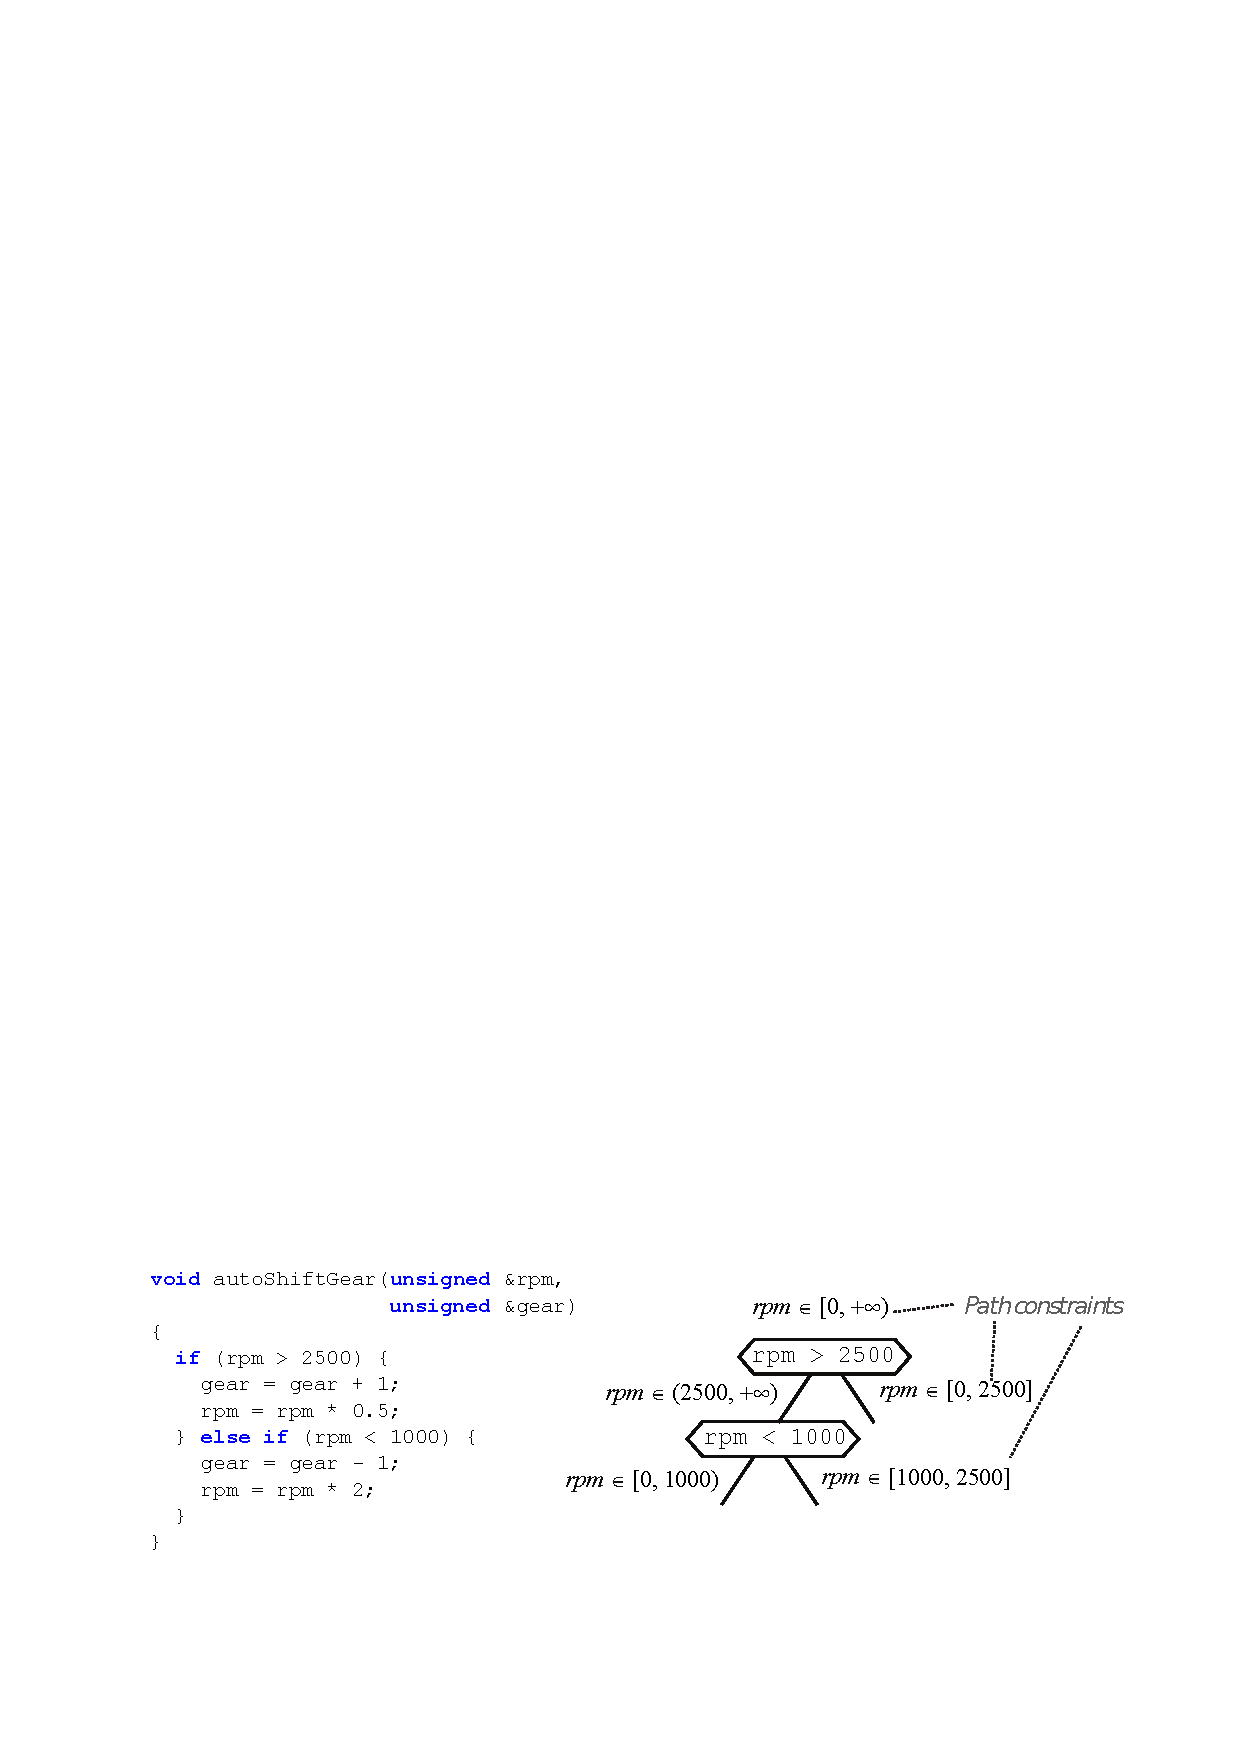
\includegraphics[width=\columnwidth]{symb_exe_2}
\caption{Execution tree with path constraints for the symbolic variable $rpm$ \cite{chip14s2e}}
\label{fig:introex}
\end{figure}

Following this procedure results in a tree-like structure of constrained symbolic expressions.
A constraint solver can now take all constraints along one execution path as input and find one concrete input (e.g., $\lambda = 5$) which would lead to the program following exactly this path.
Such results greatly alleviate writing reproducible test cases \cite{chip09sel}.

On a technical level, symbolic execution engines save state information (program memory, constraint information, ...) in a custom data structure.
Each conditional statement involving symbolic values results in a $fork$ of the program state.
The two newly created branches are completely independent and can therefore be processed in parallel.

% -------path explosion
As a consequence, the exponential growth of conditionals soon reveals scaling problems of this forking strategy.
Despite heavy research on optimisations mitigating this \textit{path explosion} problem
% \todo{ct} 
only relatively small programs ($\cong$ thousands of lines of code) can be analysed symbolically \cite{chip09sel}.

% -------interaction with env
%In addition to the path explosion problem, classical symbolic execution ... interaction with the environment...
Additionally, symbolic execution faces problems when the program under analysis \textit{interacts with its environment}.
If it calls a system library like $libc$, in theory the whole system stack including invoked libraries, operating system and drivers would have to be executed symbolically.
Considering the path explosion problem mentioned before, the resulting complexity makes such a profound analysis hardly feasible.

% --------standard sol
One way to solve this problem is to build abstract models of the program's environment \cite{klee08, nasa08}.
However, due to the complexity of real-world systems, building a model of the entire system is both tedious and unnecessary - the user usually wants to analyse one single program and not the whole system \cite{chip09sel}.

\bigskip

% -------- selective symbolic execution -------- %
In order to overcome typical problems of conventional symbolic execution, Chipounov et al.~at EPFL developed the concept of \textbf{selective symbolic execution} (\sse) \cite{chip09sel}.
Based on a virtual execution platform \sse gives users the illusion of running the entire system symbolically.
By limiting the scope of interest (i.e.~which parts of the system should be executed symbolically), users can effectively restrain the path explosion problem.
Program code within this defined scope is executed symbolically, whereas out-of-scope parts, which are irrelevant to the analysis, switch to concrete execution.
%One of the main contributions of the EPFL team around Chipounov is the transparent and consistent management of switching between symbolic and concrete execution modes.

% pruning for scalability -> bringen?

Definition of the scope of interest (what to execute symbolically) is highly flexible.
Users may specify whole executables, code regions, or even single variables to be executed symbolically. Everything else will be treated concretely.

% This forth and back conversion -> challenge!
But since on a technical level symbolic and concrete execution are handled very differently - concrete code may run natively while symbolic instructions need to be emulated - switching back and forth these two modes is a major challenge.
Hence one of the main contributions of the EPFL team around Chipounov is the transparent and consistent management of switching between symbolic and concrete execution modes.

% Bild mit Baum: single-multi-path execution

Figure \ref{fig:ssetree} depicts the \textbf{interplay of symbolic and concrete execution}.
The illustration is based on a scenario where an application $App$ is tested.
A function $appFn$ invokes the method $libFn$ in a library $Lib$, which in turn calls a function $sysFn$ in the kernel.
Since we suspect a bug in $libFn$, we focus our analysis upon this function.
Due to the path explosion problem, symbolically executing the entire system stack is not feasible.
Hence only execution inside $libFn$ follows this technique.

\medskip
\textbf{Concrete} $\rightarrow$ \textbf{symbolic transition:}
When execution enters the function $libFn$ it has to change from concrete into symbolic domain (grey areas).
This is done by replacing concrete parameters in the method call with symbolic variables.
The call $libFn(10)$ becomes $libFn(\lambda)$.\\
%, optionally also with constraints: $libFn(\lambda \le 15)$.\\
Besides the symbolic multi-path execution, \sse simultaneously also runs the function with its original concrete arguments.
This is necessary in order to return a feasible calculation result to $appFn$ and thus keep the execution of $App$ consistent.


\begin{figure}
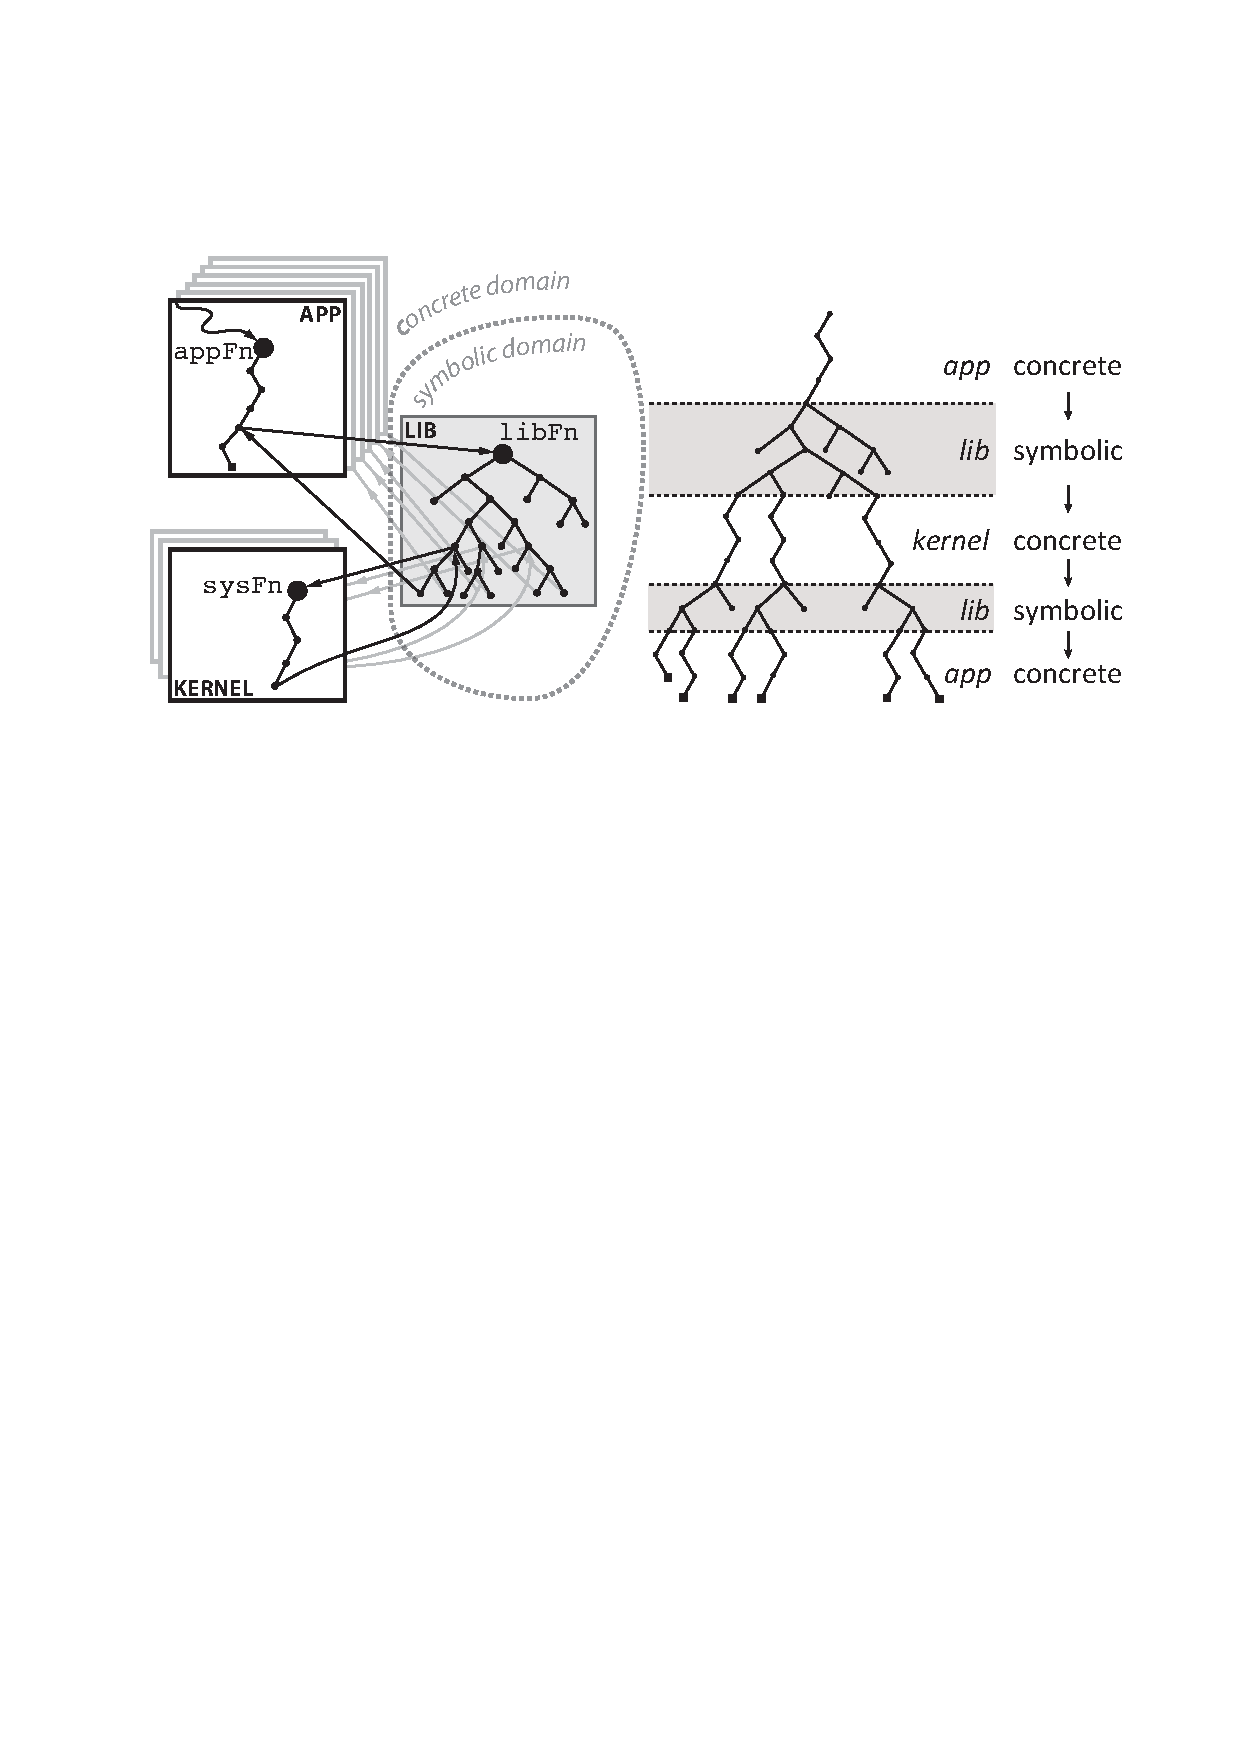
\includegraphics[width=\columnwidth]{tree}
\caption{Selective symbolic execution: only paths inside a defined scope of interest (here: a library function $libFn$) are explored symbolically - the rest of the system stack runs concretely \cite{chip14s2e}.}
\label{fig:ssetree}
\end{figure}

\medskip
\textbf{Symbolic} $\rightarrow$ \textbf{concrete transition:}
Since the operating system is not the focus of this analysis example, \sse has to switch from symbolic to concrete domain when $libFn$ calls into the kernel.
This is done by randomly picking a concrete value which fulfils all path constraints.
If, for instance, the current path is constrained with $x \in$ $]-\infty;5]$, \sse might choose $x=4$ and call $sysFn(4)$.\\
However, when $sysFn(4)$ returns, $libFn$ can no longer make any assumptions about any $x \neq 4$, because the behaviour of $sysFn$ in those cases remains unclear.
In order to preserve correctness, a new constraint $x = 4$ has to be added to the path\footnote{Constraints added because of a symbolic $\rightarrow$ concrete transition are called `soft constraints'.}.
But imagine $libFn$ being implemented as shown in figure \ref{fig:ssetree2}; now the `then' branch of the if-condition ($x < 0$) can never be reached.
Chipounov calls this effect ``overconstraining'' \cite{chip14s2e} - it is a result of concretising x when leaving the symbolic domain.
\sse tackles the problem by going back in the execution tree and forking an additional sub-tree.
The new sub-tree now picks a different concrete value for x which allows to enter the previously unreachable `then' branch.
% ----------- expand - corset - Begriffe bringen?

\begin{figure}
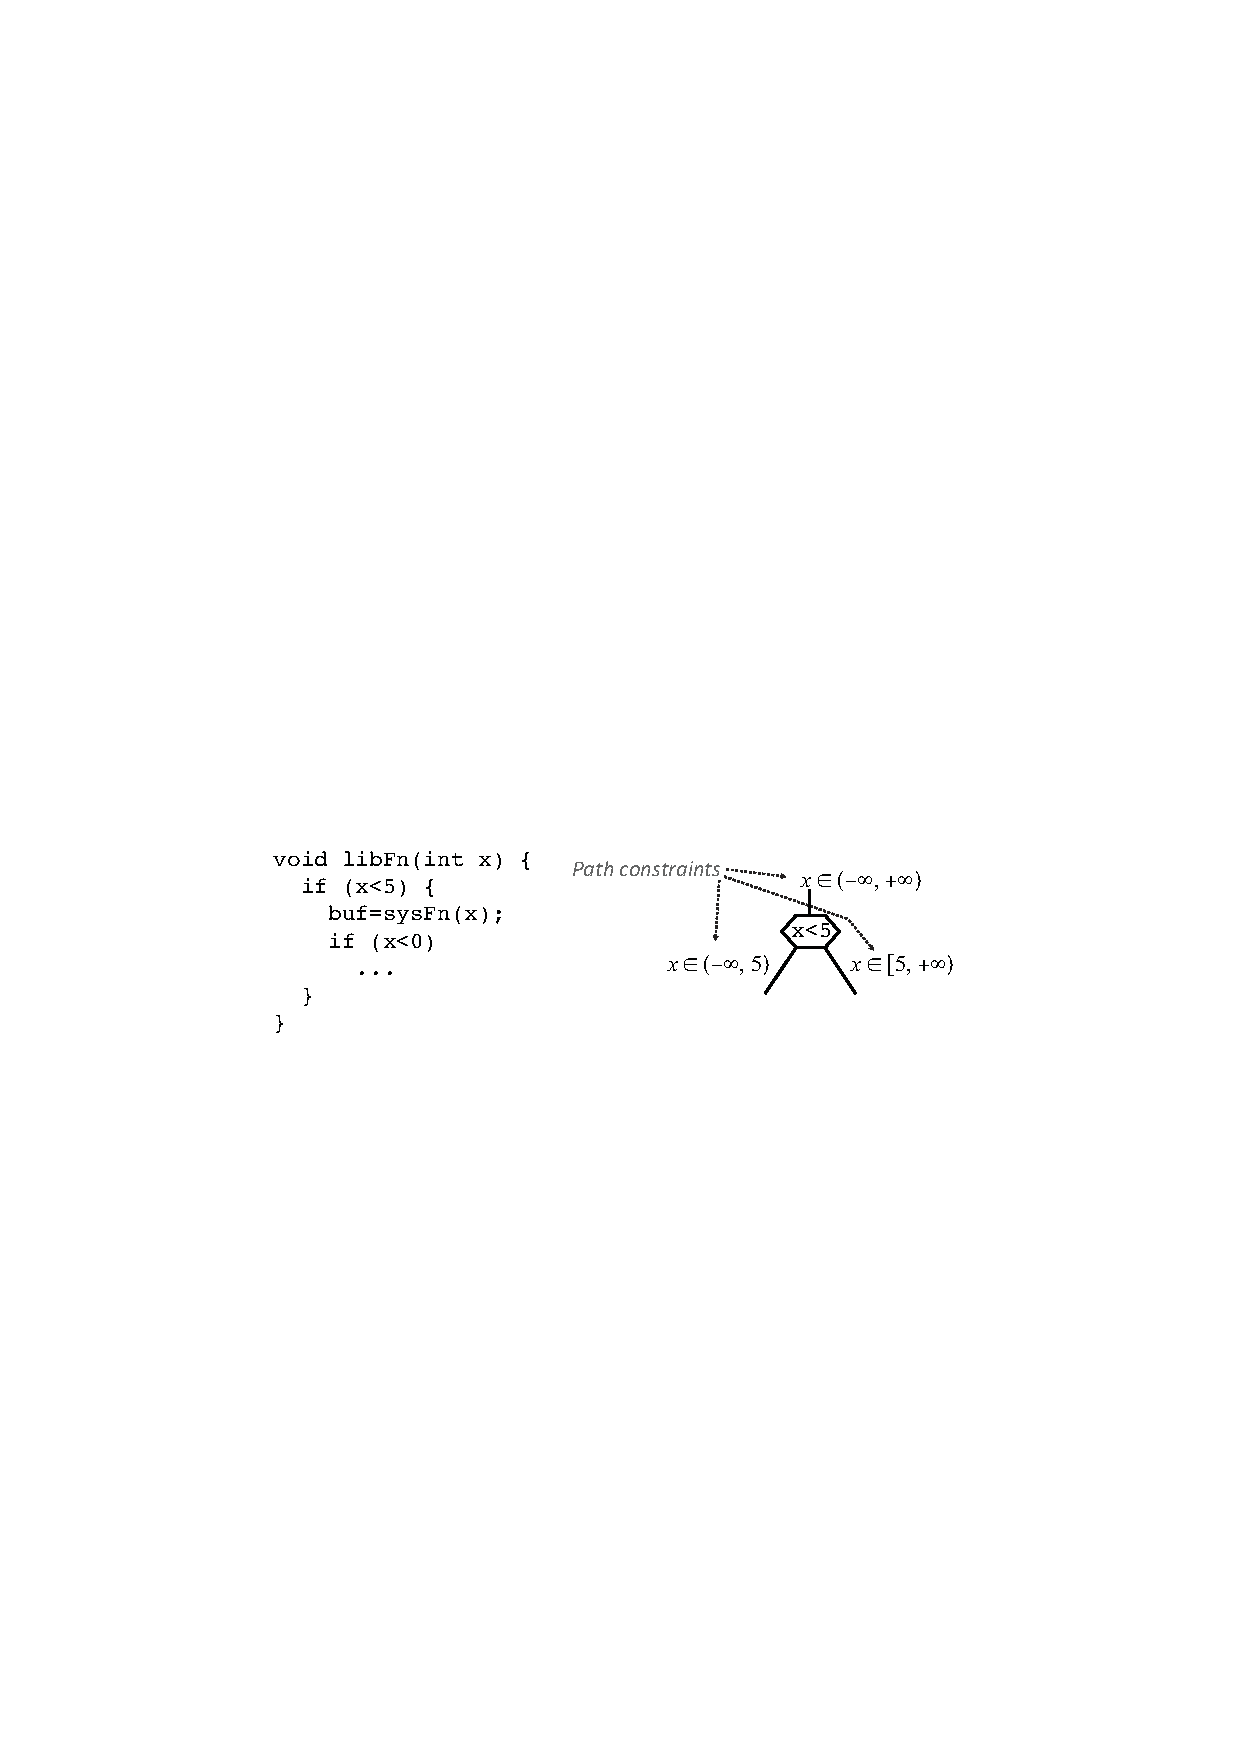
\includegraphics[width=\columnwidth]{symb_exe_space_73}
\caption{Excerpt from $libFn$'s execution tree \cite{chip12s2e}}
\label{fig:ssetree2}
\end{figure}


% -------- Konsistenzmodelle -------- %
\medskip
%Consistency models...\todo{!}
The ability to flexibly switch between symbolic and concrete execution enables \sse to handle different \textbf{execution consistency models}.
Consistency models allow to precisely control where and how to employ symbolic execution.
The user can thus strike a balance between under-approximation (only a subset of all feasible paths is explored $\rightarrow$ not complete but quick and no incorrect results) and over-approximation (a superset of all feasible paths is explored $\rightarrow$ slow but complete) of paths.
Chipounov defines six distinct consistency models.
For a basic understanding, the following paragraph will describe two of them (see \cite{chip14s2e}, p.~24ff for a detailed explanation of all models).
The first presented model (\textit{SC-CE}) describes a naive form of testing (an example of under-approximation) while the latter (\textit{RC-OC}) presents an example for a model employing over-approximation.

The most simple model is called \textit{strictly consistent concrete execution (SC-CE)}.
This is the model which is applied when testing or debugging programs either manually or with input from random test case generators (fuzzing).
`Strict consistency' describes the fact that every execution path can be mapped to concrete input values.
This model never produces false positives, i.e.~infeasible paths.


One entirely different strategy is \textit{relaxed consistency overapproximate consistency (RC-OC)}.
In this model constraints defined in API contracts can be ignored.
Under \textit{RC-OC}, a call of the system function \textit{write(fd, buf, count)} would also allow return values larger than $count$, even though that is infeasible (assuming that the C library containing the function $write()$ works correctly).
Kuznetsov et al.~\cite{kuznetsov2010testing} and Chipounov and Candea \cite{chipounov2010reverse} claim that this behaviour can be particularly useful for reverse engineering or for finding vulnerabilities in a program.
They argue that including some ``allegedly impossible hardware behaviours [...] improves the quality of the reverse engineering'' \cite[p. 11]{chip12s2e}.\\
\textit{RC-OC} is not consistent (pursues many infeasible paths) but complete (eventually finds every valid path through the system).


%%%%%%%%%%%%%%%%%%%%%%%%%%%%%%%%%%%%%%%%%%%%%%%%%%%%%%%
\iffalse
§2	Selective Symbolic Execution
		> Theorie-Teil
		> Was ist Symbolic Execution?
		> Was kann Selective Symbolic Execution besser?
			(Concrete -> symbolic transition usw.)
		> Konsistenzmodelle (wird hier evtl. schwierig, das richtige Maß 
			zu finden, um die Sache auf wenig Platz zu verstehen)
\fi
